Als een systeem langzaam aan trager aan het worden is willen we graag weten wat er aan de hand is. Met een lijst zoals door \texttt{ps} gegeven kunnen we dat lastig monitoren, omdat we niet kunnen zien wat er in de tijd gebeurd. Met \texttt{top}\index{top}\index{commando!top} kunnen we dat wel. \texttt{top} laat je in real-time zien wat er op je systeem gebeurt. Als je \texttt{top} opstart ziet het scherm er ongeveer uit zoals in figuur \ref{fig:top}.

\begin{figure}[H]
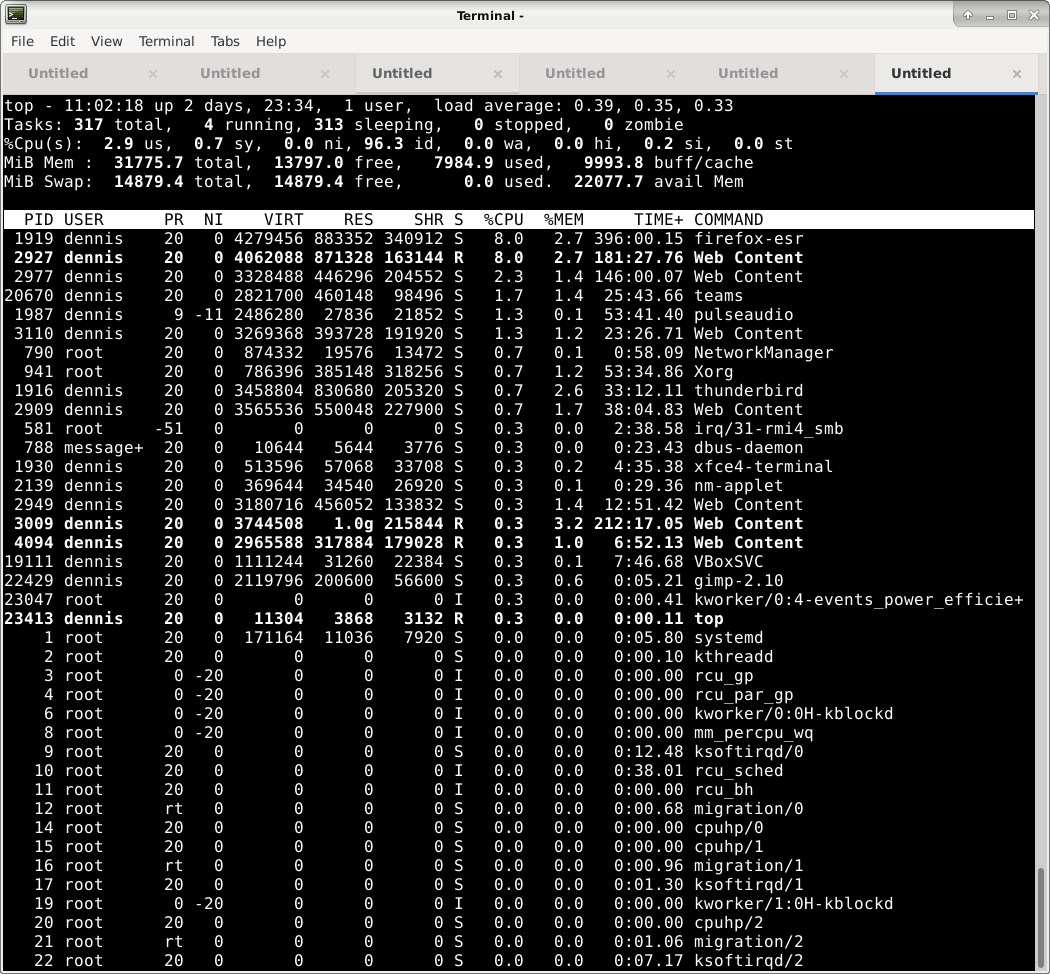
\includegraphics[width=\textwidth]{top}
\centering
\caption{Top}
\label{fig:top}
\end{figure}
Met \texttt{q} verlaten we \texttt{top}.

\texttt{top} geeft je in \'e\'en scherm heel veel informatie over je systeem en welke processen het meeste van je systeem vragen. Standaard sorteert \texttt{top} de processen op processor gebruik. We wie in het lijstje dat \texttt{firefox-esr} 8.0\% CPU gebruikt en 2.7\% van het geheugen. Met M en P (\textbf{let op} hoofdletters), kan je schakelen tussen een overzicht van het meeste processor (P) gebruik of het meeste memory (M) gebruik.
